\documentclass[a4paper,12pt]{report}

\usepackage{alltt, fancyvrb, url}
\usepackage{amssymb}
\usepackage{graphicx}
\usepackage{subfigure}
\usepackage{wrapfig}
\usepackage{algorithmic}
\usepackage[utf8]{inputenc}
\usepackage{fontenc}
\usepackage{amsmath,stmaryrd,mathtools,algorithm}
\usepackage{amssymb}
%\usepackage{amsfonts}
\usepackage{float}
\usepackage{hyperref}
\usepackage{listings}
\usepackage{url}

\usepackage[english]{cleveref}

\usepackage[english]{babel}

\newtheorem{definition}{Definition}[section]
\newtheorem{theorem}{Theorem}[section]
\newtheorem{property}{Property}[section]
\newcommand{\R}{\mathbb{R}}
\newcommand{\Z}{\mathbb{Z}}
\newcommand{\dd}{\cdot}

\title{Introduction to LLL\\``Cryptography''}
 
\author{Di Santi Giovanni}
\date{\today}

\begin{document}
 
\maketitle

\tableofcontents

\chapter{Introduction to Lattices}

\section{Vector Spaces}

\begin{definition}
    \textbf{Vector space}.
\end{definition}
A \texttt{vector space} $V$ is a subset of $\R^{m}$ which is closed under finite vector addition and scalar multiplication, with the property that

\begin{center}
   $a_1v_1 + a_2v_2 \in V$ for all $v_1,v_2 \in V$ and all $a_1,a_2 \in \R$
\end{center}

\begin{definition}
    \textbf{Linear Combinations}
\end{definition}

Let $v_1,v_2,\ldots,v_k \in V$. A \texttt{linear combination} of $v_1,v_2,\ldots,v_k \in V$ is any vector of the form

\begin{center}
    $\alpha_1v_1 + \alpha_2v_2 + \cdots + \alpha_kv_k$ with $\alpha_1, \ldots, \alpha_k \in \R$
\end{center}

\begin{definition}
    \textbf{Lineaer Independece}
\end{definition}

A set of vectors $v_1,v_2,\ldots,v_k \in V$ is \texttt{linearly independent} if the the only way to get

\begin{center}
    $a_1v_1 + a_2v_2 + \cdots + a_kv_k = 0$
\end{center}

is to have $a_1 = a_2 = \cdots = a_k = 0$.

\begin{definition}
    \textbf{Bases}
\end{definition}

Taken a set of linearly independent vectors $b = (v_1,\ldots,v_n) \in V$ we say that $b$ is a \texttt{basis} of $V$ if $\forall w \in V$ we can write

\begin{center}
    $w = a_1v_1 + a_2v_2 + \cdots + a_nv_n$
\end{center}

\begin{definition}
    \textbf{Vector's length}
\end{definition}

The vector's length or \texttt{Euclidean norm} of $v = (x_1, x_2, \ldots, x_m)$ is

\begin{center}
    $\lVert v \rVert = \sqrt{x_1^2 + x_2^2 + \cdots + x_m^2}$
\end{center}

\begin{definition}
    \textbf{Dot Product}
\end{definition}

Let $v, w \in V \subset \R^m$ and $v = (x_1, x_2, \ldots, x_m), w = (y_1, y_2, \ldots, y_m)$, the \texttt{dot product} of $v$ and $m$ is

\begin{center}
    $v \dd m = x_1y_1 + x_2y_2 + \cdots + x_my_m$

    or

    $v \dd m = \lVert v \rVert \lVert w \rVert \cos{\theta}$
\end{center}

where $\theta$ is the angle between $v$ and $w$ if we place the starting points of the vectors at the origin $O$.

\begin{figure}[!b]
    \centering
    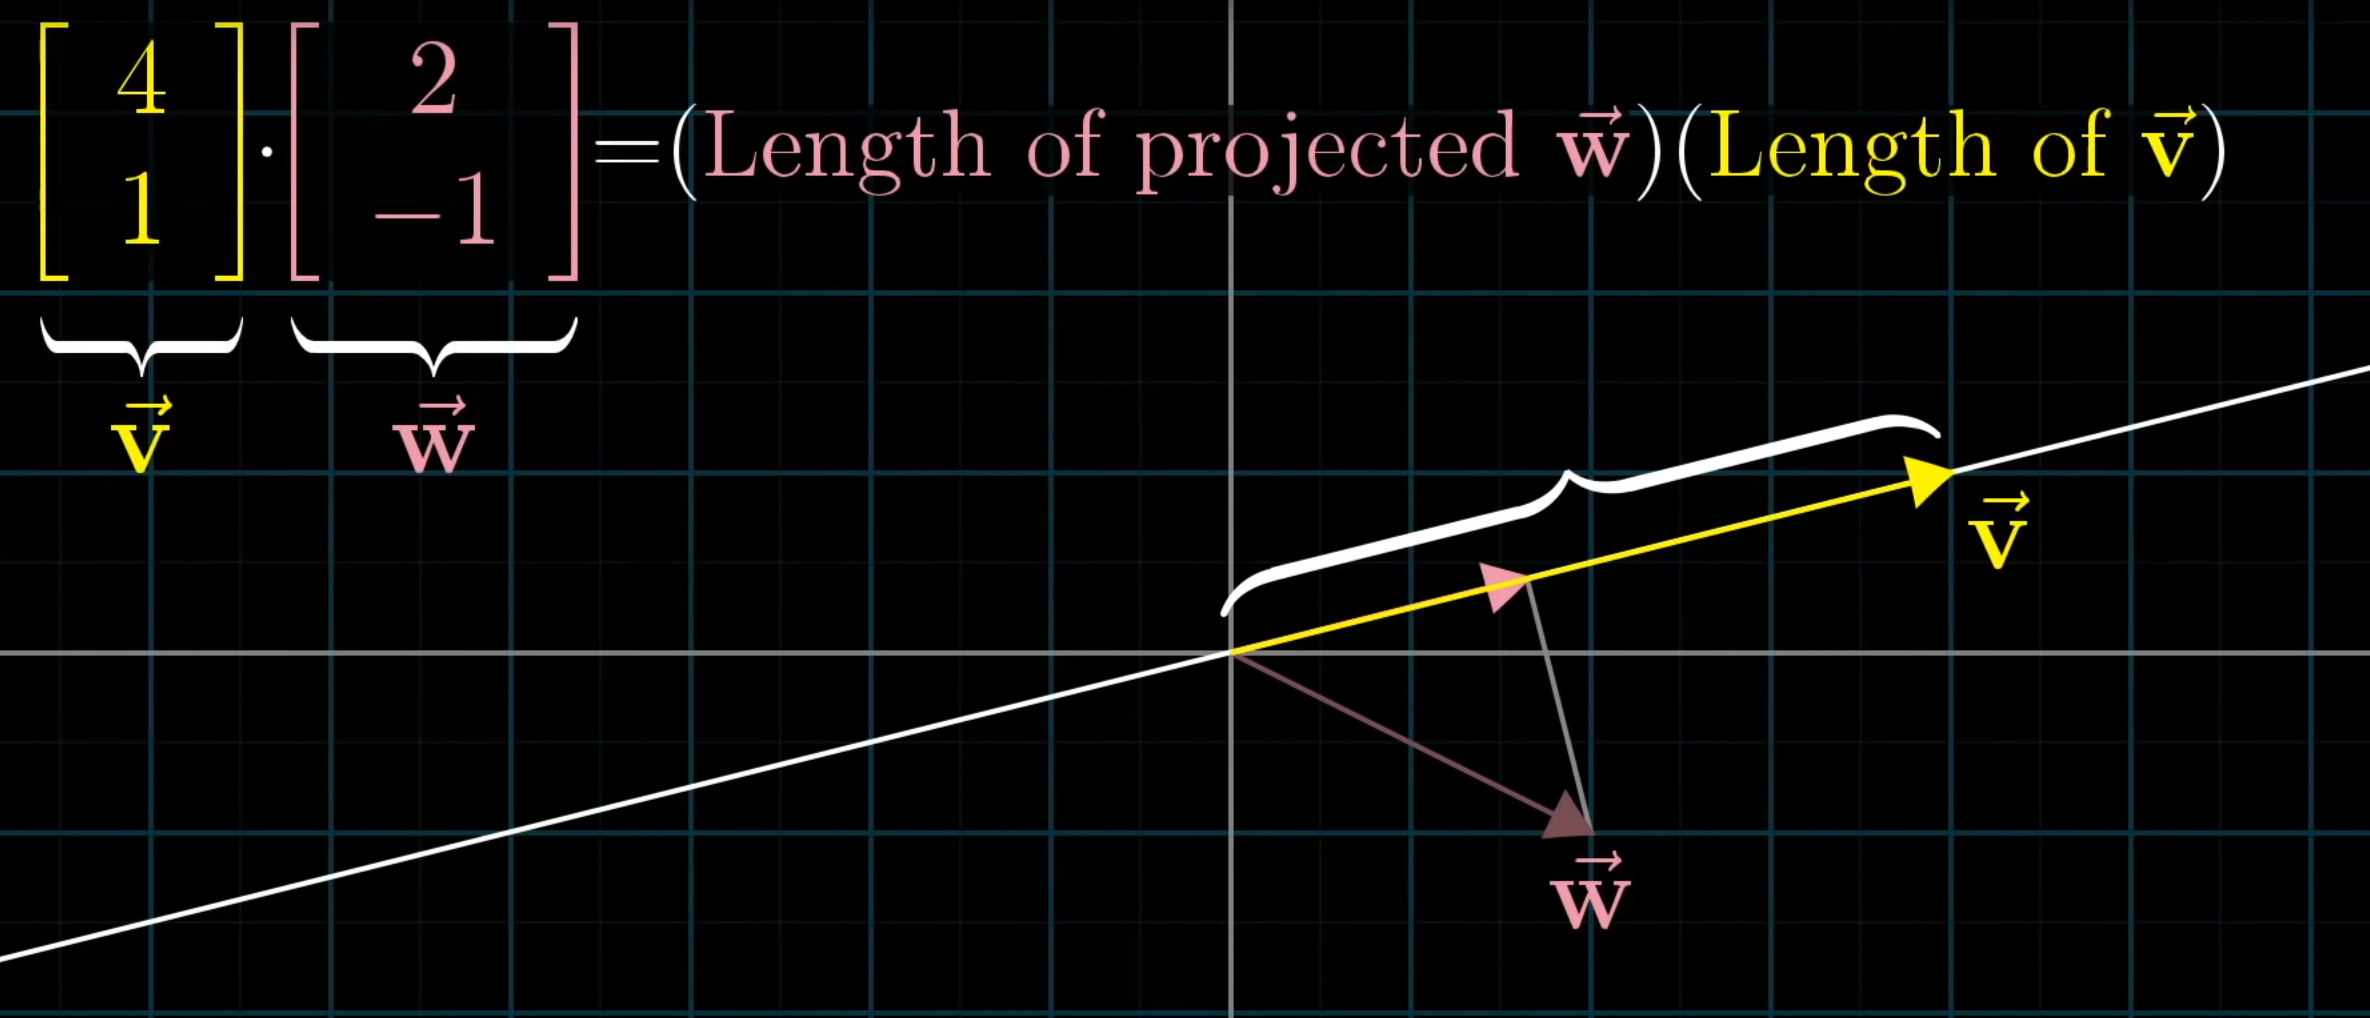
\includegraphics[scale=0.2]{./img/dot_product.png}
    \caption{Dot Product By 3Blue1Brown}
    \label{fig:dot_product}
\end{figure}

Geometrically speaking $v \cdot m$ is the length of $w$ projected to $v$ multiplied by the length of $v$ as shown in \ref{fig:dot_product}

\begin{definition}
    \textbf{Ortoghonal Basis} 
\end{definition}

An \texttt{ortoghonal basis} for a vector space $V$ is a basis $v_1, \ldots, v_m$ with the property that

\begin{center}
    $v_i \dd v_j = 0$ for all $i \neq j$
\end{center}

If $\lVert v_i \rVert = 1$ for all $i$ then the basis is \texttt{orthonormal}.

\begin{algorithm}
    \textbf{Gram-Schmidt Algorithm}
\end{algorithm}

Let $b = (v_1, \ldots, v_n)$, be a basis for a vector space $V \subset \R^m$. There is an algorithm to create an orthogonal basis
$b^* = (v_1^*,\ldots,v_n^*)$.
The two bases have the property that Span$\{v_1,\ldots,v_i\}$ = Span$\{v_1^*,\ldots,v_i^*\}$ for all $i = 1,2,\ldots,n$

\begin{figure}[htpb]
    \centering
    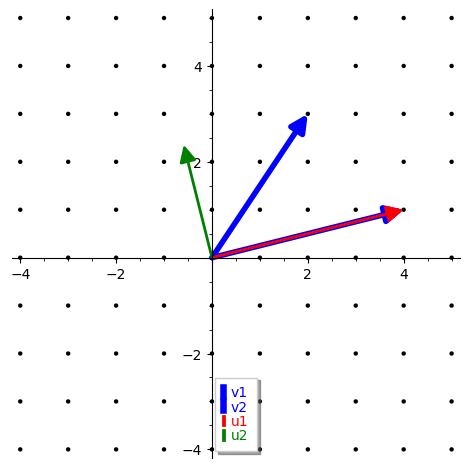
\includegraphics[width=0.5\textwidth]{./img/gram_schmidt.png}
    \caption{Gram Schmidt orthogonalization}
    \label{fig:gram_schmidt}
\end{figure}

If we take $v_1=(4, 1), v_2=(2, 3)$ as basis and apply gram schmidt we obtain $u_1=v_1=(4, 1), u_2=(-10/17, 40/17)$ as shown in \ref{fig:gram_schmidt}

\section{Lattices}

\begin{definition}
    \textbf{Lattice}
\end{definition}

Let $v_1,\ldots,v_n \in \R^m, m \ge n$ be linearly independent vectors. A \texttt{Lattice} $L$ spanned by $\{v_1,\ldots,n_n\}$ is the set of 
all integer linear combinations of $v_1,\ldots,v_n$.

\begin{center}
    $L = \bigg\{\sum_{i=1}^{n} a_iv_i, a_i \in \Z \bigg\}$
\end{center}

If $v_i$ for every $i = 1,\ldots\,n$ has integer coordinates then the lattice is
called \texttt{Integral Lattice}.

On the figure \ref{fig:lattice0} we show a lattice $L$ with bases $v=(3, 1)$ and $w=(-1, 1)$, and on \ref{fig:lattice1} the same lattice $L$ with
a different basis.

\begin{figure}[!tbp]
    \begin{minipage}[b]{0.50\textwidth}
        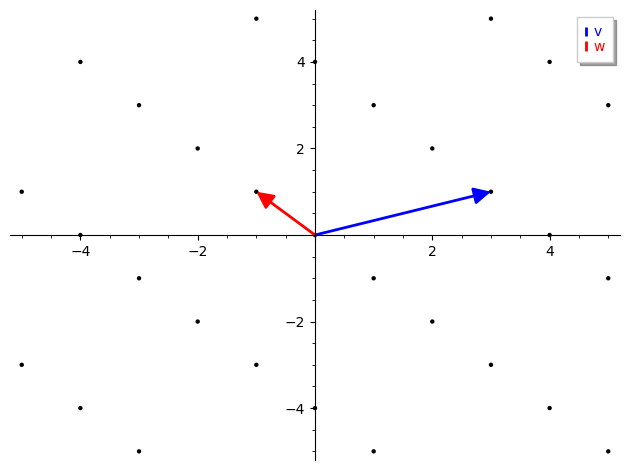
\includegraphics[width=\textwidth]{./img/lattice_b0.png}
        \caption{Lattice $L$ spanned by $v, w$}
        \label{fig:lattice0}
    \end{minipage}
    \hspace{\fill}
    \hspace{\fill}
    \hspace{\fill}
    \hspace{\fill}
    \hspace{\fill}
    \begin{minipage}[b]{0.50\textwidth}
        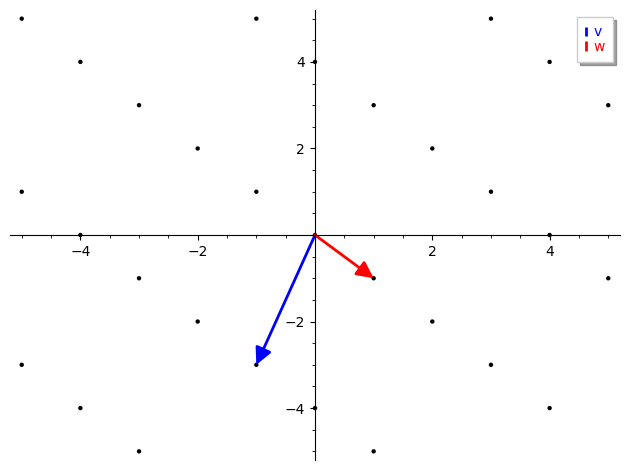
\includegraphics[width=\textwidth]{./img/lattice_b1.png}
        \caption{Lattice $L$ spanned by $v', w'$}
        \label{fig:lattice1}
    \end{minipage}
\end{figure}

\section{Problems}

\subsection{SVP}

\textbf{The Shortest Vector Problem} (\texttt{SVP}): Find a nonzero vector $v \in L$ that minimez the Euclidean norm $\lVert v \rVert$.

\begin{algorithm}
    \textbf{Gauss Reduction}
\end{algorithm}

Gauss's developed an algorithm to find an optimal basis for a two-dimensional lattice given an arbitrary basis. The output of the algorithm
gives the shortest nonzero vector in $L$ and in this way solves the \texttt{SVP}.

If we take for example $v_1 = (10, 4), v_2 = (7, 5)$ and apply the gauss reduction algorithm we
obtain $w_1 = (3, -1), w_2 = (4, 6)$ \ref{fig:gauss_svp}. $w_1$ is the shortest nonzero vector in the lattice $L$ spanned by $v_1, v_2$.

\begin{figure}[b]
    \centering
    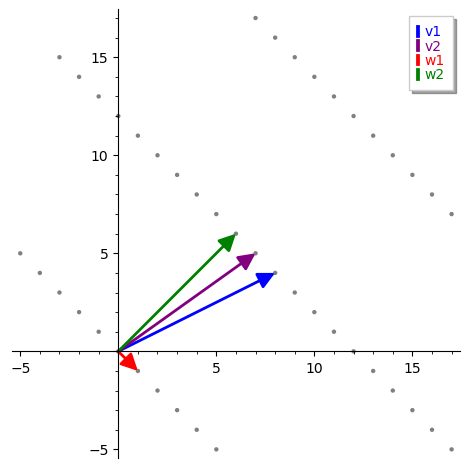
\includegraphics[width=0.5\textwidth]{./img/gauss_svp.png}
    \caption{Gauss reduction}
    \label{fig:gauss_svp}
\end{figure}

However the bigger the dimension of the lattice, the harder is the problem and there isn't a polynomial algorithm to find such vector.

\subsection{CVP}

\textbf{The Closest Vector Problem} (\texttt{CVP}): Given a vector $w \in \R^m$ that is not in $L$, find a vector $v \in L$ that is closest to $w$,
in other words find a vector $v \in L$ that minimizes the Euclidean norm $\lVert w - v \rVert$.

Example in \ref{fig:cvp}

\begin{figure}[t]
    \centering
    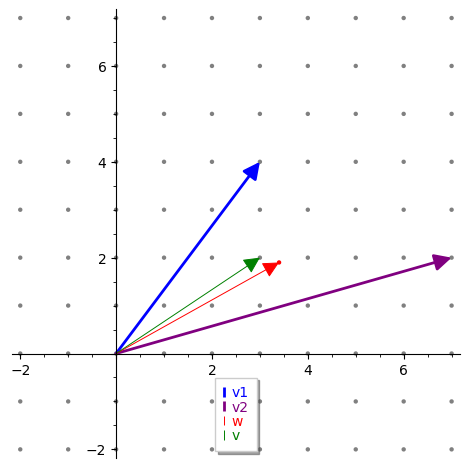
\includegraphics[width=0.5\textwidth]{./img/cvp.png}
    \caption{CVP}
    \label{fig:cvp}
\end{figure}

% matrix([[0, 0, 1], [1, 1, 2], [1, 2, 1]])
\chapter{LLL}

\section{Purpose}

\section{Algorithm}

\chapter{Applications}

\section{Attack Knapsack}

\section{Attack RSA}

\chapter*{End of Paper}

$gg^2$

\bibliographystyle{plain}
\bibliography{paper}

\end{document}

